In this section, the layer is described in some detail in terms of its specific subsystems. Describe each of the layers and its subsystems in a separate chapter/major subsection of this document. The content of each subsystem description should be similar. Include in this section any special considerations and/or trade-offs considered for the approach you have chosen.

\begin{figure}[h!]
	\centering
 	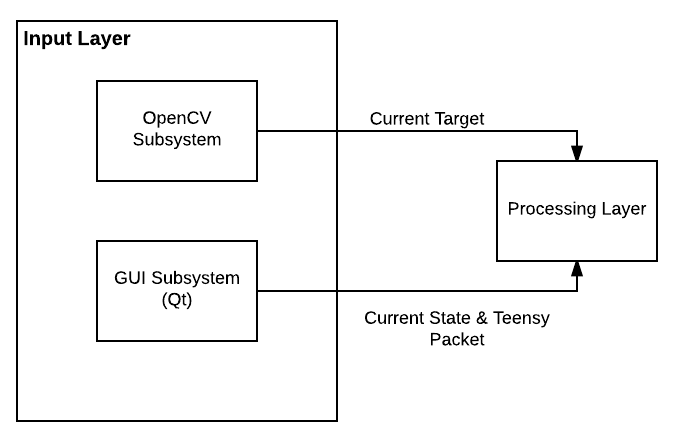
\includegraphics[width=0.60\textwidth]{images/input}
 \caption{Input Layer subsystem diagram}
\end{figure}

\subsection{GUI Subsystem (Qt)}
The purpose of the GUI subsystem is to provide an interface for the user to operate and control the system, as well as see its processes.

\subsubsection{Assumptions}
The GUI should be able to show the camera feed as well as the OpenRave simulation on the screen, and should be able to receive and send this information

\subsubsection{Responsibilities}
The GUI subsystem will be responsible for rendering and displaying the user interface, along with the live camera feed and the Openrave simulation. This UI will also generate events to the system when the user interacts with anything interactible on the interface.

\subsubsection{Subsystem Interfaces}


\begin {table}[H]
\caption {GUI interfaces} 
\begin{center}
    \begin{tabular}{ | p{1cm} | p{6cm} | p{3cm} | p{3cm} |}
    \hline
    ID & Description & Inputs & Outputs \\ \hline
    \#1 & Data gets stored as a data packet to send to the Processing Layer & \pbox{3cm}{Event generated by the application} & \pbox{3cm}{None}  \\ \hline

    \end{tabular}
\end{center}
\end{table}

\subsection{OpenCV Subsystem}
The OpenCV Subsystem is what is able to take and show the camera feed.

\subsubsection{Assumptions}
The OpenCV subsystem will be able to take the camera feed and be able to determine the current target to give to the processing layer.

\subsubsection{Responsibilities}
The OpenCV subsystem will be responsible for processing the camera feed and accurately pinpointing the target for the arm and send that data to the processing layer.

\subsubsection{Subsystem Interfaces}


\begin {table}[H]
\caption {OpenCV interfaces} 
\begin{center}
    \begin{tabular}{ | p{1cm} | p{6cm} | p{3cm} | p{3cm} |}
    \hline
    ID & Description & Inputs & Outputs \\ \hline
    \#1 & Data sent from the camera feed & \pbox{3cm}{Camera feed} & \pbox{3cm}{Sent to OpenRave subsystem}  \\ \hline

    \end{tabular}
\end{center}
\end{table}